
\documentclass[12pt,a4paper]{article}
\usepackage[utf8]{inputenc}
\usepackage[T1]{fontenc}
\usepackage[a4paper,margin=2.2cm]{geometry}
\usepackage{setspace}
\usepackage{xcolor}
\usepackage{booktabs}
\usepackage{longtable}
\usepackage{array}
\usepackage{listings}
\usepackage{hyperref}
\usepackage{tikz}
\usetikzlibrary{arrows.meta,positioning,shapes.geometric,calc}
\usepackage{caption}
\usepackage{enumitem}
\setstretch{1.12}
\setlength{\parindent}{0pt}
\setlength{\parskip}{6pt}
\setlist[itemize]{topsep=3pt,itemsep=2pt,parsep=0pt}
\setlist[enumerate]{topsep=3pt,itemsep=2pt,parsep=0pt}
\hypersetup{colorlinks=true,linkcolor=blue!55!black,citecolor=blue!55!black,urlcolor=blue!55!black}
\definecolor{softgray}{RGB}{245,245,245}
\definecolor{linegray}{RGB}{70,70,70}
\lstdefinestyle{jsonstyle}{basicstyle=\ttfamily\small,backgroundcolor=\color{softgray},frame=single,rulecolor=\color{linegray},breaklines=true,showstringspaces=false,tabsize=2}
\lstset{style=jsonstyle}
\newcommand{\code}[1]{\texttt{#1}}
\newcommand{\formalcover}[4]{%
\begin{titlepage}
\centering
\vspace*{1.2cm}
{\Large Universitat Autonoma de Barcelona}\\[4pt]
{\large Master Degree in Modelling for Science and Engineering}\\[4pt]
{\large Institution / Lab: IIIA-CSIC}\\[2.0cm]
{\Huge\bfseries #1}\\[0.35cm]
{\Large #2}\\[1.5cm]
{\large Formal architecture and contract section for technical review.}\\[2.0cm]
\begin{tabular}{>{\bfseries}p{0.28\linewidth}p{0.58\linewidth}}
Document type: & Architecture and contract walkthrough\\
Academic year: & 2025--2026\\
Date: & #3\\
Scope: & #4\\
Repository: & \url{https://github.com/ieverythng/nao-ros4hri-bridge}\\
\end{tabular}
\vfill
\end{titlepage}}

\begin{document}

\formalcover{Technical Memory Draft Baseline}{End-to-End Planner Dialogue Flow: Supervisor-Integrated Revision}{2026-06-03}{Runtime flow, ROS contracts, compact grounding, planner output, feedback, and dialogue ownership.}

\section{End-to-End User to Planner Dialogue Flow}

\subsection{Purpose}

This document is the supervisor-facing and thesis-facing walkthrough for the active planner stack. It describes the path from a user utterance to robot execution and spoken feedback, with emphasis on which node owns each decision. The document is payload-oriented, but the payloads are intentionally simplified so that they describe the current minimal architecture rather than speculative future seams.

The central design principle is that the LLM planner is not a robot controller. The chatbot extracts the user's goal and compact context; the planner proposes a structured plan over known skills; the orchestrator validates and dispatches executable steps; skills refresh live evidence before reporting outcomes; and the dialogue manager realizes speech. Figure~\ref{fig:corrected-runtime-flow} shows this runtime responsibility chain.

\subsection{End-to-End Runtime Flow}

\begin{figure}[h]
\centering
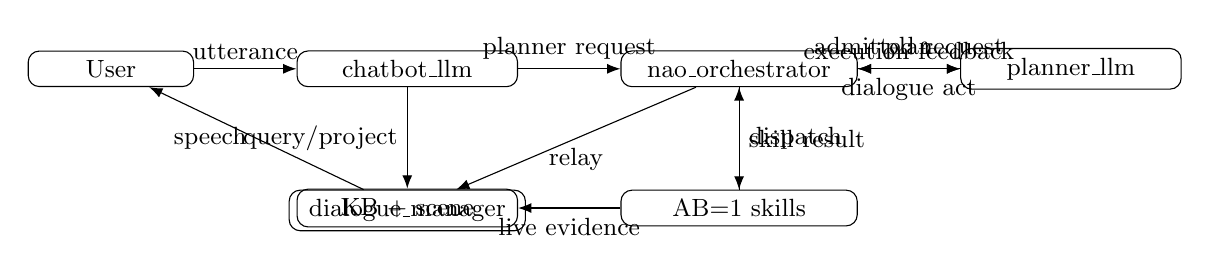
\begin{tikzpicture}[node distance=1.3cm,>=Latex,every node/.style={font=\small}]
\node[draw,rounded corners,align=center,minimum width=2.1cm] (u) {User};
\node[draw,rounded corners,align=center,right=of u,minimum width=2.8cm] (c) {chatbot\_llm};
\node[draw,rounded corners,align=center,right=of c,minimum width=3.0cm] (o) {nao\_orchestrator};
\node[draw,rounded corners,align=center,right=of o,minimum width=2.8cm] (p) {planner\_llm};
\node[draw,rounded corners,align=center,below=of o,minimum width=3.0cm] (s) {AB=1 skills};
\node[draw,rounded corners,align=center,left=of s,minimum width=2.8cm] (k) {KB + scene};
\node[draw,rounded corners,align=center,below=of c,minimum width=3.0cm] (d) {dialogue\_manager};
\draw[->] (u) -- node[above]{utterance} (c);
\draw[->] (c) -- node[above]{planner request} (o);
\draw[->] (o) -- node[above]{admitted request} (p);
\draw[->] (p) -- node[above]{plan} (o);
\draw[->] (o) -- node[right]{dispatch} (s);
\draw[->] (s) -- node[below]{live evidence} (k);
\draw[->] (s) -- node[right]{skill result} (o);
\draw[->] (o) -- node[above]{execution feedback} (p);
\draw[->] (p) -- node[below]{dialogue act} (o);
\draw[->] (o) -- node[below]{relay} (d);
\draw[->] (d) -- node[left]{speech} (u);
\draw[->] (c) -- node[left]{query/project} (k);
\end{tikzpicture}
\caption{Runtime message flow and responsibility assignment from user input to spoken response. The chatbot extracts the user's goal and compact context, the orchestrator admits planner requests and dispatches executable steps, the planner generates and supervises structured plans, AB=1 skills refresh live KB/scene evidence, and the dialogue manager realizes user-facing speech.}
\label{fig:corrected-runtime-flow}
\end{figure}

The term \emph{turn} refers to one dialogue exchange initiated by a user utterance and processed by the dialogue stack. A turn may remain conversational, answer a KB query, or produce a planner request.

\subsection{Contract Map}

Table~\ref{tab:corrected-contract-map} lists the runtime interfaces in the current architecture. All rows refer either to ROS topics/actions/services or to JSON payloads carried in ROS message fields.

\begin{longtable}{p{0.24\linewidth}p{0.31\linewidth}p{0.20\linewidth}p{0.19\linewidth}}
\caption{Runtime contracts and ownership in the active planner stack.}\label{tab:corrected-contract-map}\\
\toprule
Contract & ROS interface or payload location & Producer & Consumer\\
\midrule
Chatbot turn output & internal chatbot result before ROS publication & \code{chatbot\_llm} & planner handoff logic\\
Planner request & \code{/nao\_orchestrator/planner\_request} and \code{/planner/request}; payload in \code{Intent.data} & \code{chatbot\_llm}, admitted by \code{nao\_orchestrator} & \code{planner\_llm}\\
Compact grounding & \code{Intent.data.grounded\_context} in the planner request & \code{chatbot\_llm} & \code{planner\_llm}\\
Planner output & \code{/intents}; payload in \code{Intent.data.plan} & \code{planner\_llm} & \code{nao\_orchestrator}\\
Skill execution & ROS actions exposed by AB=1 skill servers & \code{nao\_orchestrator} & skill servers\\
Execution feedback & \code{/planner/execution\_feedback}; JSON string payload & \code{nao\_orchestrator} & \code{planner\_llm}\\
Planner dialogue act & \code{/planner/dialogue\_act} and orchestrator relay topic & \code{planner\_llm} & \code{dialogue\_manager} via orchestrator\\
Raw KB/scene evidence & \code{/scene/summary}, \code{/kb/query}, tracked-person feeds, skill results & scene, KB, and skills & chatbot projection and skill-local checks\\
\bottomrule
\end{longtable}

\subsection{Chatbot Turn Output}

The intent in this contract is the user's goal as extracted by the chatbot: what the robot is being asked to achieve. It is not a planner output.

\begin{lstlisting}
{
  "verbal_ack": "Okay, I will do that.",
  "route": "execution",
  "confidence": 0.82,
  "user_intent": {
    "type": "look_at",
    "goal_text": "look at the person",
    "scene_targets": ["person"],
    "request_kind": "new_goal"
  }
}
\end{lstlisting}

\begin{longtable}{p{0.28\linewidth}p{0.62\linewidth}}
\caption{Fields in the chatbot turn output.}\label{tab:chatbot-fields}\\
\toprule
Field & Meaning\\
\midrule
\code{verbal\_ack} & Optional immediate acknowledgement generated by the chatbot layer.\\
\code{route} & Classification of the turn as \code{dialogue}, \code{knowledge\_query}, or \code{execution}. Only \code{execution} turns enter the planner path.\\
\code{confidence} & Confidence assigned by the chatbot/intention extraction stage. It is not a planner priority.\\
\code{user\_intent.type} & Normalized user-intent label extracted by the chatbot.\\
\code{user\_intent.goal\_text} & Natural-language objective passed to the planner as the task to satisfy.\\
\code{user\_intent.scene\_targets} & Optional target hints extracted from the utterance, such as \code{person} or \code{cup}.\\
\code{user\_intent.request\_kind} & Goal transition class: new goal, update, clarification answer, or cancellation.\\
\bottomrule
\end{longtable}

\subsection{Compact Grounding and Knowledge Snapshot}

The planner receives a compact, JSON-native view of relevant world state. This is best described as a compact scene graph derived from KB rows, scene summaries, and tracked people. It replaces earlier separate descriptions of \code{knowledge\_snapshot}, \code{scene\_summary}, and \code{state\_t0} for the default planner prompt. Raw KB triples and detector metadata remain available to skills, but they are not duplicated into every LLM prompt.

\begin{lstlisting}
{
  "grounded_context": {
    "entities": [
      {
        "id": "cup_jrjic",
        "label": "cup",
        "kind": "object",
        "class": "Cup",
        "visible": true,
        "relations": [
          {"predicate": "dbp:color", "object": "blue"},
          {"predicate": "oro:isOn", "object": "table_1"}
        ]
      },
      {
        "id": "anonymous_person_ehfbf",
        "label": null,
        "kind": "person",
        "class": "Human",
        "visible": true,
        "relations": []
      }
    ]
  }
}
\end{lstlisting}

\begin{longtable}{p{0.24\linewidth}p{0.66\linewidth}}
\caption{Fields in compact grounding.}\label{tab:grounding-fields}\\
\toprule
Field & Meaning\\
\midrule
\code{id} & Stable entity handle used by planner steps and skill arguments.\\
\code{label} & Human-readable name or class hint. It may be empty for anonymous people.\\
\code{kind} & Entity category, currently \code{object} or \code{person}. This avoids treating people as generic objects.\\
\code{class} & Compact semantic class used by the planner for reasoning.\\
\code{visible} & Whether the entity is currently grounded in perception.\\
\code{relations} & Prioritized semantic relations that add information beyond the class, such as color or containment.\\
\bottomrule
\end{longtable}

The compact view should omit detector score, image coordinates, backend, source, and recency by default. Those values are execution evidence, not planning semantics, unless a future skill explicitly needs them in its own action arguments.

\subsection{Planner Request}

The planner request is the minimal task description admitted by the orchestrator and consumed by the planner. It should not contain a requested plan: if the system is requesting a plan, it should not prefill the plan in the same message.

\begin{lstlisting}
{
  "goal_id": "goal_turn_123",
  "request_kind": "new_goal",
  "goal_text": "look at the person and report completion",
  "normalized_intents": ["look_at"],
  "grounded_context": {
    "entities": [
      {
        "id": "anonymous_person_ehfbf",
        "label": null,
        "kind": "person",
        "class": "Human",
        "visible": true,
        "relations": []
      }
    ]
  }
}
\end{lstlisting}

\begin{longtable}{p{0.28\linewidth}p{0.62\linewidth}}
\caption{Fields in the minimal planner request.}\label{tab:planner-request-fields}\\
\toprule
Field & Meaning\\
\midrule
\code{goal\_id} & Identifier for the user's active objective. It groups replans and feedback for the same task.\\
\code{request\_kind} & Transition type. \code{new\_goal} creates a new objective; \code{clarification\_answer} continues a waiting objective; \code{cancel\_request} cancels it.\\
\code{goal\_text} & Objective extracted from the user's utterance. This is the central planning input.\\
\code{normalized\_intents} & Chatbot-derived intent labels used as hints for selecting admissible skills.\\
\code{grounded\_context} & Compact scene graph used by the planner to resolve entities and avoid purely language-prior planning.\\
\bottomrule
\end{longtable}

Fields such as \code{request\_id}, \code{dialogue\_turn\_id}, \code{planner\_mode}, parent lineage, and supersede lineage can remain implementation metadata when needed by traces or admission logic, but they are not part of the minimal thesis-level planner contract unless the experiment explicitly evaluates them.

\subsection{Planner LLM Internals}

After the planner request is admitted, \code{planner\_llm} builds a prompt from the minimal request, compact grounding, the skill registry, allowed step types, and the output contract. Rule-based shortcuts may produce deterministic plans for simple motions. Otherwise, the LLM provider returns JSON, which is parsed and validated before publication. Invalid JSON or unsupported steps trigger a validation retry or a failure result.

\subsection{Planner Output}

The planner output is a plan: a sequence of skill steps to achieve the user goal. It should focus on executable content and minimal lineage. Communication policy and retry metadata may be kept only if the runtime uses them; otherwise they should be omitted from the thesis-level contract.

\begin{lstlisting}
{
  "plan": {
    "goal_id": "goal_turn_123",
    "plan_id": "plan_123",
    "plan_version": 1,
    "status": "planned",
    "steps": [
      {
        "id": "step_1",
        "type": "skill",
        "name": "look_at",
        "args": {"target_frame": "anonymous_person_ehfbf"},
        "requires": [],
        "on_failure": "replan"
      }
    ]
  }
}
\end{lstlisting}

\begin{longtable}{p{0.28\linewidth}p{0.62\linewidth}}
\caption{Fields in the planner output.}\label{tab:planner-output-fields}\\
\toprule
Field & Meaning\\
\midrule
\code{goal\_id} & User objective that this plan attempts to satisfy.\\
\code{plan\_id} & Identifier for this concrete plan proposal. It is useful only if the runtime keeps plan history.\\
\code{plan\_version} & Revision number for replans of the same goal.\\
\code{status} & Planning result, for example \code{planned}, \code{needs\_clarification}, or \code{failed\_to\_plan}.\\
\code{steps} & Ordered skill calls produced by the planner. This is the essential output.\\
\code{steps[].id} & Stable step identifier used for feedback and possible replan joins.\\
\code{steps[].name} & Skill name selected from the allowed registry.\\
\code{steps[].args} & Skill arguments. They should refer to known entity IDs or explicit primitive values.\\
\code{steps[].requires} & Dependencies between steps, if any.\\
\code{steps[].on\_failure} & Requested recovery policy for the step, such as \code{replan} or \code{fail}.\\
\bottomrule
\end{longtable}

If the planner cannot produce a plan, the output should represent that as a planning result rather than filling the plan with ambiguous failure fields. For the simple version, \code{steps} is the most important field.

\subsection{Scan and Report Evidence Flow}

The planner may produce a \code{scan} step followed by \code{report\_result}. The planner should not fabricate the report from stale prompt context. The scan skill owns fresh perception, and \code{report\_result} reports the latest live skill result.

\begin{lstlisting}
{
  "plan": {
    "goal_id": "goal_turn_123",
    "status": "planned",
    "steps": [
      {
        "id": "step_1",
        "type": "skill",
        "name": "scan",
        "args": {"target_kind": "objects"},
        "requires": [],
        "on_failure": "replan"
      },
      {
        "id": "step_2",
        "type": "skill",
        "name": "report_result",
        "args": {},
        "requires": ["step_1"],
        "on_failure": "fail"
      }
    ]
  }
}
\end{lstlisting}

This distinction is central to avoiding a node-ownership mismatch: the planner selects \emph{what} skill should run, while the skill and orchestrator determine the current evidence and what can be truthfully reported.

\subsection{Execution Feedback}

For the simple version, execution feedback can be minimal. The planner needs to know which goal is affected, which step failed or succeeded, and a compact result if that result is useful for replanning or dialogue. A large feedback payload is only justified if the planner actually consumes the extra fields.

\begin{lstlisting}
{
  "goal_id": "goal_turn_123",
  "status": "failed",
  "step": {
    "id": "step_1",
    "name": "look_at"
  },
  "reason": "target frame unavailable",
  "result_payload": {
    "target_found": false,
    "target_kind": "person"
  }
}
\end{lstlisting}

\begin{longtable}{p{0.28\linewidth}p{0.62\linewidth}}
\caption{Fields in minimal execution feedback.}\label{tab:feedback-fields}\\
\toprule
Field & Meaning\\
\midrule
\code{goal\_id} & User objective affected by the feedback.\\
\code{status} & Outcome of the executed step or plan segment.\\
\code{step.id} & Step identifier from the planner output. This is the key field for replanning.\\
\code{step.name} & Skill name that produced the feedback.\\
\code{reason} & Short explanation of the outcome, especially for failure.\\
\code{result\_payload} & Optional structured evidence that the planner can use for replanning or clarification.\\
\bottomrule
\end{longtable}

\subsection{Planner Dialogue Act}

Planner dialogue acts represent planner intent to communicate, not direct speech execution. They are relayed through the orchestrator and realized by the dialogue layer.

\begin{lstlisting}
{
  "goal_id": "goal_turn_123",
  "act": "ask_clarification",
  "await_user_response": true,
  "reason": "multiple visible people",
  "text_hint": "Which person should I look at?",
  "slots_needed": ["target_person"]
}
\end{lstlisting}

Allowed dialogue acts are acknowledgement, progress update, clarification, help request, failure explanation, completion notification, and cancellation notification. The planner does not speak directly; it emits a structured communication request.

\subsection{Replanning and Join Semantics}

The current conceptual policy is a single active-goal model. \code{goal\_id} preserves continuity of the user's objective, while \code{plan\_id} and \code{plan\_version} are only necessary if the runtime tracks multiple plan attempts for the same goal. Replanning should use stable \code{step.id} values: if the current step can be mapped into the new plan, the executor may mid-join; otherwise it should resume from the first pending compatible step.

\subsection{Live Supervisor Demo Script}

\begin{enumerate}
\item Trigger one execution command and show the chatbot output with \code{route=execution}.
\item Show the compact \code{grounded\_context} on the planner request.
\item Show the admitted request on \code{/planner/request}.
\item Show planner output on \code{/intents} and highlight \code{steps}, the most important field.
\item Run one scan/report case and show that \code{report\_result.args} is empty.
\item Run one failure or clarification path.
\item Show the minimal execution feedback and the resulting dialogue act.
\item Close with the ownership map: chatbot extracts and grounds, planner plans, orchestrator dispatches, skills provide live evidence, dialogue manager speaks.
\end{enumerate}

\end{document}
